%% Copyright 2023 P. S. Eduardo.
%
% This work may be distributed and/or modified under the
% conditions of the LaTeX Project Public License, either version 1.3
% of this license or (at your option) any later version.
% 
% The Current Maintainer of this work is P. S. Eduardo.
%
% This work consists of the file poli.cls.
%% -----------------------------------------------------------------
% Escola Politécnica UFRJ LaTeX Template
% Version: 2302
% Author: Eduardo Paiva dos Santos
% email: eduardopaiva@poli.ufrj.br
% Base: CoppeTeX 2.3
%%------------------------------------------------------------------
\documentclass[grad,pdftex]{poli}
\usepackage[utf8]{inputenc}
\usepackage{amsmath,amssymb}
\usepackage{float}
\usepackage{multirow}
\usepackage{longtable}
\usepackage{tikz}
\usetikzlibrary{shapes,arrows,chains,positioning}
\usepackage{enumitem}
\usepackage{indentfirst}
\usepackage{array}
\usepackage{diagbox}
\usepackage{natbib}

%\usepackage[alf, bibjustif]{abntex2cite}

\makelosymbols
\makeloabbreviations

\begin{document}
  \title{Título do TCC}
  \foreigntitle{TCC Title}
  \author{Nome}{Sobrenome}
  \advisor{Prof.}{Nome}{Sobrenome}{D.Sc.}
  %\coadvisor{Prof.}{Nome}{Sobrenome}{D.Sc.}
  \examiner{Prof.}{Nome Completo}{Ph.D.}
  \examiner{Prof.}{Nome Completo}{D.Sc.}
  %\examiner{Prof.}{Nome Completo}{D.Sc.}
  \department{DEL} %UTTILIZE A SIGLA DO SEU DEPARTAMENTO MODIFICAR OS NOMES DE CURSO, DEPARTAMENTO E OBTENÇÃO DE GRAU (Obs: caso tenha algum equívoco nesses argumentos, necessário modificar o arquivo poli.cls no local que faz a leitura deste argumento)
  \date{11}{2023}
  \keyword{keyword1}
  \keyword{keyword2}
  \keyword{keyword3}
  \keyword{keyword4}
  \maketitle

  \frontmatter
  \dedication{``Acreditar que você pode sarrar já é meio caminho para sarrada'' - Autor desconhecido.}


  \chapter*{Agradecimentos}

Agradeça seus pais, seus professores, seus amigos e eu acreditando que ninguém fosse ler esse capítulo, mas no meu TCC teve professor corrigindo texto aqui rsrsr.
  \begin{abstract}

Fale sobre os objetivos do seu trabalho e brevemente como você fez para alcança-los. Apresente alguns \textit{highlights} dos seus resultados obtidos.

\end{abstract}


  \begin{foreignabstract}

Se tu não manja do \textit{english}, mete um google tradutor que safa

\end{foreignabstract}


  \tableofcontents
  \listoffigures
  \listoftables
  \printlosymbols
  \printloabbreviations

  \mainmatter
    \chapter{Introdução}

\section{Lorem Ipsum}

Lorem ipsum dolor sit amet, consectetur adipiscing elit. Nunc et rutrum tortor. Aenean placerat sed erat at posuere. Praesent a dui augue. Etiam ultrices est in eleifend convallis. Nulla condimentum eleifend nunc, quis commodo nisi imperdiet a. Vestibulum dolor neque, rutrum ac cursus vitae, facilisis et felis. Nam magna massa, molestie ut luctus et, blandit et odio. Vestibulum dignissim, magna quis ultrices convallis, felis sem tempus orci, nec lacinia nibh massa a nulla. Suspendisse potenti. Fusce bibendum tortor quis quam scelerisque sollicitudin. Ut a tempor orci, vel efficitur ante.

Aenean purus arcu, auctor sed interdum vel, feugiat a lacus. Fusce nec nibh quis ipsum maximus finibus in at nulla. In non ultricies felis, ac interdum mi. Fusce eu congue sem. Nam congue aliquam libero, nec bibendum mi sollicitudin non. Suspendisse cursus ligula vitae nunc finibus, sed eleifend enim vestibulum. Proin facilisis leo rhoncus nisl hendrerit interdum. Aenean est ligula, gravida eget nunc et, vehicula pharetra dui. In eu massa egestas, auctor ante non, consequat odio. (\cite{alvim2007}).

Curabitur rhoncus blandit ipsum, id consequat urna venenatis id. Aliquam ex nisi, vestibulum quis tellus quis, ultricies egestas orci. Donec eu libero dui. Integer elementum felis et ligula congue rutrum. Sed a feugiat purus, eu rutrum massa. Vestibulum commodo elit id ornare pharetra. Pellentesque at pretium diam. Morbi sit amet placerat justo. Cras id nulla eros. Donec iaculis ligula eu gravida porttitor. Vestibulum tristique dapibus arcu porta euismod. Ut bibendum at nunc et interdum. In egestas pretium lacus, ut aliquet ipsum ultrices quis. Morbi euismod justo arcu, consequat sagittis orci aliquam in. Vivamus dignissim, libero vel accumsan viverra, odio erat venenatis sapien, a gravida quam neque vitae nisi.(\cite{mme2020}). 

\begin{figure}[H]
    \centering
    
\includegraphics[width=0.5\linewidth]{Imagens/chap01/loren-ipsum-cover.jpg}
    \caption{Maecenas viverra convallis sem, id imperdiet neque rhoncus et. Ut vel mi erat. Nam quam arcu, mollis sodales felis at, sagittis iaculis lectus.}
    \label{fig:lorem_ipsum}
\end{figure}

\section{Organização do TCC}

In ornare, enim non porta interdum no Capítulo \ref{chap2},est lorem volutpat metus, pellentesque pharetra lacus est sed lacus. Vivamus quis magna et justo mattis commodo viverra in tellus. (Apêndice \ref{apendice}).

Aliquam convallis mauris sit amet elementum condimentum. Vestibulum eget tellus massa. Aenean nisl tortor, consequat ac lacus maximus, hendrerit consequat purus. Fusce aliquam, leo vel dictum molestie, lorem nibh aliquam diam, sit amet accumsan justo ante sit amet tellus no Capítulo \ref{chap6}.
    \chapter{Revisão Bibliográfica}
\label{chap2}

\section{Lorem Ipsum}

Lorem ipsum dolor sit amet, consectetur adipiscing elit. Nunc et rutrum tortor. Aenean placerat sed erat at posuere. Praesent a dui augue. Etiam ultrices est in eleifend convallis. Nulla condimentum eleifend nunc, quis commodo nisi imperdiet a. Vestibulum dolor neque, rutrum ac cursus vitae, facilisis et felis. Nam magna massa, molestie ut luctus et, blandit et odio. Vestibulum dignissim, magna quis ultrices convallis, felis sem tempus orci, nec lacinia nibh massa a nulla. Suspendisse potenti. Fusce bibendum tortor quis quam scelerisque sollicitudin. Ut a tempor orci, vel efficitur ante.

\begin{figure}[H]
  \centering
  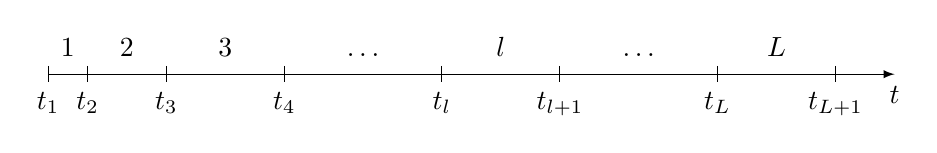
\begin{tikzpicture}
    % draw horizontal line   
    \draw (0,0) -- (0.5,0);
    \draw (0.5,0) -- (1.5,0);
    \draw (1.5,0) -- (3,0);
    \draw (3,0) -- (5,0);
    \draw (5,0) -- (6.5,0);
    \draw (6.5,0) -- (8.5,0);
    \draw (8.5,0) -- (10,0);



    % draw vertical lines
    \foreach \x in {0,0.5,1.5,3,5,6.5,8.5,10}
      \draw (\x cm,3pt) -- (\x cm,-3pt);
      
    \draw[-latex] (10,0) -- (10.75,0) node[below=1pt] {$ t $};      

    % draw nodes
    \draw (0,0) node[below=3pt] {$ t_1 $};
    \draw (0.25,0) node[above=3pt] {$ 1 $};
    \draw (0.5,0) node[below=3pt] {$ t_2 $};
    \draw (1,0) node[above=3pt] {$ 2 $};
    \draw (1.5,0) node[below=3pt] {$ t_3 $}; 
    \draw (2.25,0) node[above=3pt] {$ 3 $};
    \draw (3,0) node[below=3pt] {$ t_4 $};
    \draw (4,0) node[above=3pt] {$ \ldots $};
    \draw (5,0) node[below=3pt] {$ t_l $};
    \draw (5.75,0) node[above=3pt] {$ l $};
    \draw (6.5,0) node[below=3pt] {$ t_{l+1} $};
    \draw (7.5,0) node[above=3pt] {$ \ldots $};
    \draw (8.5,0) node[below=3pt] {$ t_L $};
    \draw (9.25,0) node[above=3pt] {$ L $};
    \draw (10,0) node[below=3pt] {$ t_{L+1} $};
    \draw (10.75,0);
  \end{tikzpicture}
  \label{chap2:timeline}
  %\vspace{-1cm}
  \caption{Intervalos de queima.}  
  \end{figure}

Lorem ipsum dolor sit amet, consectetur adipiscing elit. Nunc et rutrum tortor. Aenean placerat sed erat at posuere. Praesent a dui augue. Etiam ultrices est in eleifend convallis.

\begin{equation}
    \phi_g(\vec{r},t) \cong \phi_g(\vec{r},t_l) \quad \text{para} \quad t \in [t_l,t_{l+1}).
\end{equation}

Aenean purus arcu, auctor sed interdum vel, feugiat a lacus. Fusce nec nibh quis ipsum maximus finibus in at nulla. In non ultricies felis, ac interdum mi Equação \ref{chap2:iso:1}: 

\begin{equation}
    \frac{d}{dt}\underline{N}^n(t) = E_l^n \underline{N}^n(t_l) \quad \text{para} \quad t_l \leq t \leq t_{l+1} \quad l =1,\ldots,L,
    \label{chap2:iso:1}
\end{equation}

\noindent{}com 

\begin{equation*}
    \underline{N}^n(t) \equiv 
    \begin{bmatrix}
    N_1^n(t) \\
    N_2^n(t) \\
    \vdots \\
    N_i^n(t) \\
    \vdots \\
    N_I^n(t)
    \end{bmatrix}.
\end{equation*}    
    \chapter{Metodologia Proposta}
\label{chap3}

\section{Lorem Ipsum}

Lorem ipsum dolor sit amet, consectetur adipiscing elit. Nunc et rutrum tortor. Aenean placerat sed erat at posuere. Praesent a dui augue. Etiam ultrices est in eleifend convallis. Nulla condimentum eleifend nunc, quis commodo nisi imperdiet a. Vestibulum dolor neque, rutrum ac cursus vitae, facilisis et felis. Nam magna massa, molestie ut luctus et, blandit et odio. Vestibulum dignissim, magna quis ultrices convallis, felis sem tempus orci, nec lacinia nibh massa a nulla. Suspendisse potenti. Fusce bibendum tortor quis quam scelerisque sollicitudin. Ut a tempor orci, vel efficitur ante.

\begin{enumerate}
    \item Para a obtenção de $b_{3gu}^n(t_l)$:
    
    \begin{equation}
    \begin{split}
        \left[12D_g^n(t_l)/(a_u^n)^2 + \frac{1}{5}\Sigma_{Rg}^n(t_l)\right]b_{3gu}^n(t_l) - \frac{1}{5}\left[\nu\Sigma_{fg}^n(t_l)\sum_{g'=1}^G\chi_{g'}b_{3g'u}^n(t_l)\right. + \\
        + \left.\sum_{g'=1}^G \Sigma_{g'g}^n(t_l)b_{3g'u}^n(t_l) + \right] = -\frac{1}{3}\left[\Sigma_{Rg}^n(t_l)b_{1gu}^n(t_l) + \nu\Sigma_{fg}^n(t_l)\sum_{g'=1}^G\chi_{g'}b_{1g'u}^n(t_l)\right. + \\
        \left.+\sum_{g'=1}^G\Sigma_{g'g}^n(t_l)b_{1g'u}^n(t_l)+  +\alpha_{1gu}^n(t_l)\right];
    \label{chap3:58}
    \end{split}
    \end{equation}
    
    \item Para a obtenção de $b_{4gu}^n(t_l)$:
    
    \begin{equation}
    \begin{split}
        \left[12D_g^n(t_l)/(a_u^n)^2 + \frac{3}{35}\Sigma_{Rg}^n(t_l)\right]b_{4gu}^n(t_l) - \frac{3}{35}\left[\nu\Sigma_{fg}^n(t_l)\sum_{g'=1}^G\chi_{g'}b_{4g'u}^n(t_l)\right. + \\
        \left.+ \sum_{g'=1}^G \Sigma_{g'g}^n(t_l)b_{4g'u}^n(t_l) + \right] = -\frac{1}{5}\left[\Sigma_{Rg}^n(t_l)b_{2gu}^n(t_l) + \nu\Sigma_{fg}^n(t_l)\sum_{g'=1}^G\chi_{g'}b_{2g'u}^n(t_l) \right. + \\
        +\left.\sum_{g'=1}^G\Sigma_{g'g}^n(t_l)b_{2g'u}^n(t_l)-\alpha_{2gu}^n(t_l) \right].
    \label{chap3:59}
    \end{split}        
    \end{equation}    
    
    
\end{enumerate}

\section{O Cálculo do Parâmetro de Subcriticalidade Utilizando o Método NEM}

Lorem ipsum dolor sit amet, consectetur adipiscing elit. Nunc et rutrum tortor. Aenean placerat sed erat at posuere. Praesent a dui augue. Etiam ultrices est in eleifend convallis. Nulla condimentum eleifend nunc, quis commodo nisi imperdiet a. Vestibulum dolor neque, rutrum ac cursus vitae, facilisis et felis.

\begin{table}[H]
\centering
\caption{Produto dos polinômios de base do NEM.}
\label{chap3:ksub:table}
\vspace{0.5cm}
\begin{tabular}{|>{\centering} m{2cm}|>{\centering} m{2cm}|>{\centering} m{2cm}|>{\centering} m{2cm}|>{\centering\arraybackslash} m{2cm}|}
\hline
\diagbox[innerwidth=2cm]{$m$}{$k$}        & \textbf{1}    & \textbf{2}    & \textbf{3}     & \textbf{4}      \\ \hline 
\textbf{1} & $\frac{1}{3}$ & $0$           & $\frac{1}{5}$  & $0$             \\ \hline 
\textbf{2} & $0$           & $\frac{1}{5}$ & $0$            & $-\frac{3}{35}$ \\ \hline
\textbf{3} & $\frac{1}{5}$ & $0$           & $\frac{6}{35}$ & $0$             \\ \hline
\textbf{4} & $0$           & $0$           & $0$            & $\frac{6}{105}$ \\ \hline
\end{tabular}
\end{table}


\section{Fluxograma do Algoritmo de Solução do Parâmetro de Subcriticalidade}
\label{chap3:sec:fluxograma}

A Figura \ref{chap3:fluxograma} In ornare, enim non porta interdum, est lorem volutpat metus, pellentesque pharetra lacus est sed lacus. Vivamus quis magna et justo mattis commodo viverra in tellus. Cras tempor ullamcorper libero vitae tristique. Morbi malesuada posuere tincidunt. Integer accumsan egestas ante eget elementum. Vestibulum ante ipsum primis in faucibus orci luctus et ultrices posuere cubilia curae; Curabitur ac lacinia urna. Vivamus id nunc a nisl tincidunt efficitur eget quis neque. Praesent quis lorem rhoncus, rhoncus dui vel, condimentum dolor. Curabitur condimentum augue dignissim turpis consectetur venenatis.

\begin{figure}[H]

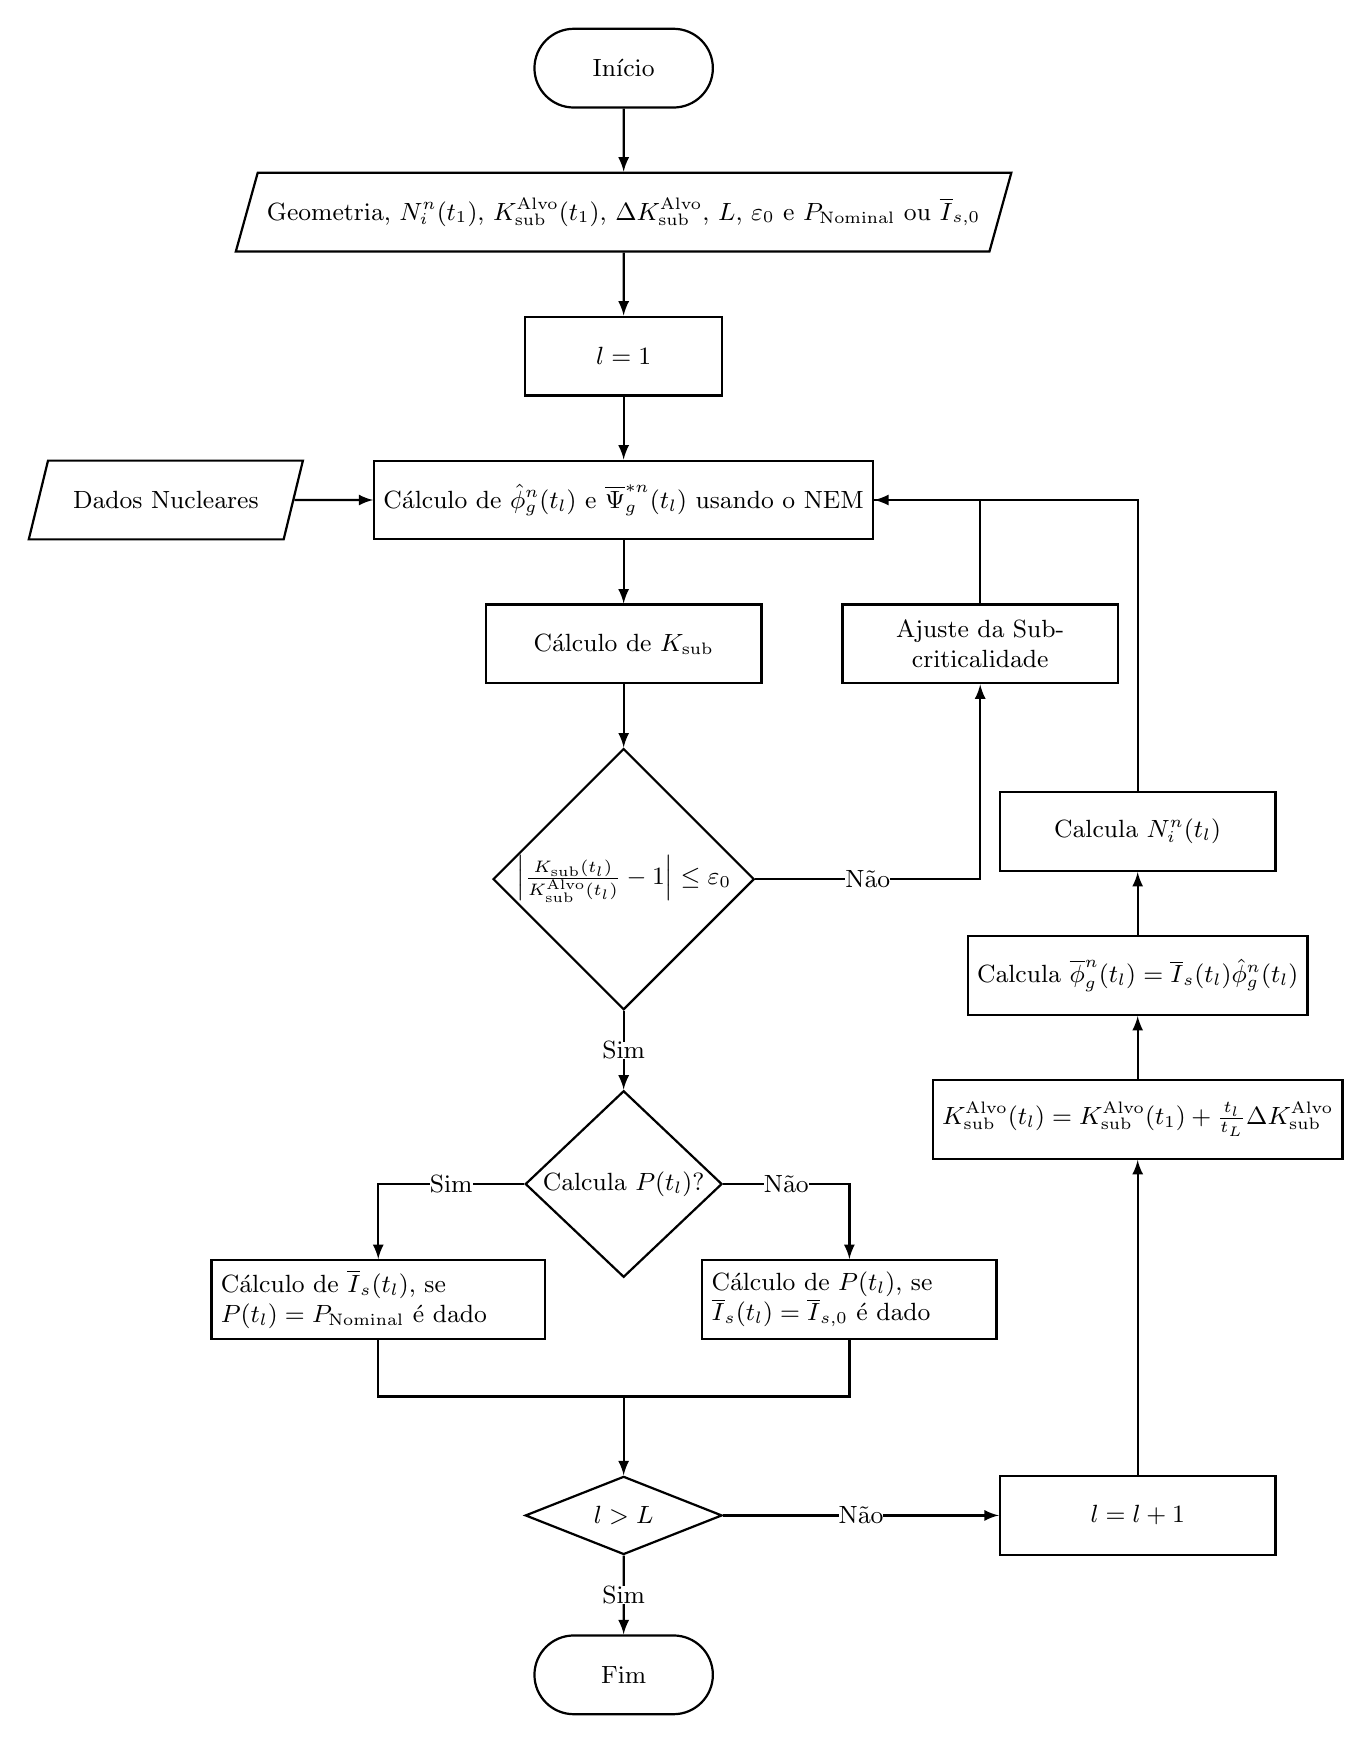
\begin{tikzpicture}[font=\small,thick]
 
% Start block
\node[draw,
    rounded rectangle,
    minimum width=2.5cm,
    minimum height=1cm] (block1) {Início};
 
% Voltage and Current Measurement
\node[draw,
    trapezium, 
    trapezium left angle = 65,
    trapezium right angle = 115,
    trapezium stretches,
    below= 0.8cm of block1,
    minimum width=3.5cm,
    minimum height=1cm
] (block2) { Geometria, $N_i^n{(t_1)}$, $K_{\text{sub}}^\text{Alvo}(t_1)$, $\Delta K_{\text{sub}}^\text{Alvo}$, $L$, $\varepsilon_0$ e $P_\text{Nominal}$ ou $\overline{I}_{s,0}$};
 
% Power and voltage variation
\node[draw,
    below=0.8cm of block2,
    minimum width=2.5cm,
    minimum height=1cm
] (block3) { $l=1$};

% Power and voltage variation
\node[draw,
    below=0.8cm of block3,
    minimum width=3.5cm,
    minimum height=1cm
] (block4) {Cálculo de $\hat{\phi}_g^n(t_l)$ e $\overline{\Psi}_g^{*n}(t_l)$ usando o NEM};

% Voltage and Current Measurement
\node[draw,
    trapezium, 
    trapezium left angle = 65,
    trapezium right angle = 115,
    trapezium stretches,
    left=of block4,
    minimum width=3.5cm,
    minimum height=1cm
] (block21) {Dados Nucleares};

% Power and voltage variation
\node[draw,
    below=0.8cm of block4,
    minimum width=3.5cm,
    minimum height=1cm
] (block5) {Cálculo de $K_{\text{sub}}$};
    
% Conditions test
\node[draw,
    diamond,
    below=0.8cm of block5,
    minimum width=2.5cm,
    inner sep=0] (block6) {$\left|\frac{K_{\text{sub}}(t_l)}{K_{\text{sub}}^\text{Alvo}(t_l)} -1 \right| \le \varepsilon_0$};
    
    
% Conditions test
\node[draw,
    diamond,
    below=of block6,
    minimum width=2.5cm,
    inner sep=0] (block7) {Calcula $P(t_l)$?};   

% Power and voltage variation
\node[draw,
    below left=0.5cm of block7,
    minimum width=3.5cm,
    minimum height=1cm,
    text width=4cm
] (block8) {Cálculo de $\overline{I}_s(t_l)$, se $P(t_l)=P_\text{Nominal}$ é dado};  

% Power and voltage variation
\node[draw,
    below right=0.5cm of block7,
    minimum width=3.5cm,
    minimum height=1cm,
    text width=3.5cm
] (block9) {Cálculo de $P(t_l)$, se $\overline{I}_s(t_l)=\overline{I}_{s,0}$ é dado};  

% Power and voltage variation
\node[draw,
    right= 1cm of block5,
    minimum width=3.5cm,
    minimum height=1cm,
    text width=3cm,
    text centered
] (block17) {Ajuste da Subcriticalidade};  

\node[coordinate,below=1.5cm of block7] (block16) {};

% Conditions test
\node[draw,
    diamond,
    below= of block16,
    minimum width=2.5cm,
    inner sep=0] (block10) {$l>L$};
  

%\node[coordinate,right=0.5cm of block17] (block18) {};
    

% Power and voltage variation
\node[draw,
    right=3.5cm of block10,
    minimum width=3.5cm,
    minimum height=1cm
] (block12) {$l=l+1$};

% Power and voltage variation
\node[draw,
    above=4cm of block12,
    minimum width=3.5cm,
    minimum height=1cm
] (block13) {$K_{\text{sub}}^\text{Alvo}(t_l) = K_{\text{sub}}^\text{Alvo}(t_1) + \frac{t_l}{t_L}\Delta K_\text{sub}^\text{Alvo}$}; 

% Power and voltage variation
\node[draw,
    above=0.8cm of block13,
    minimum width=3.5cm,
    minimum height=1cm
] (block14) {Calcula $\overline{\phi}_g^n(t_l) = \overline{I}_s(t_l)\hat{\phi}_g^n(t_l)$};    


% Power and voltage variation
\node[draw,
    above=0.8cm of block14,
    minimum width=3.5cm,
    minimum height=1cm
] (block18) {Calcula $N_i^n(t_l)$};    
    
% Return block
\node[draw,
    rounded rectangle,
    below=of block10,
    minimum width=2.5cm,
    minimum height=1cm,] (block11) {Fim};
 
% \node[coordinate,below=4.35cm of block4] (block12) {};
 
 
% Arrows
\draw[-latex] (block1) edge (block2)
    (block2) edge (block3)
    (block3) edge (block4)
    (block21) edge (block4)
    (block4) edge (block5)	
    (block5) edge (block6);
 
\draw[-latex] (block6) -- (block7)
    node[pos=0.5,fill=white,inner sep=0]{Sim};
    
\draw[-latex] (block6) -| (block17)
    node[pos=0.25,fill=white,inner sep=0]{Não};    
 
\draw[-latex] (block7) -| (block8)
    node[pos=0.25,fill=white,inner sep=0]{Sim};

\draw[-latex] (block7) -| (block9)
    node[pos=0.25,fill=white,inner sep=0]{Não};

\draw (block8) |- (block16);
 
\draw (block9) |- (block16);

\draw[-latex] (block16) -- (block10);

\draw[-latex] (block10) -- (block11)
    node[pos=0.5,fill=white,inner sep=0]{Sim};

\draw[-latex] (block10) -- (block12)
    node[pos=0.5,fill=white,inner sep=0]{Não};


\draw[-latex] (block12) edge (block13)
              (block13) edge (block14)
              (block18) |- (block4)
              (block17) |- (block4)
              (block14) edge (block18);
%\draw (block17) -- (block18);              
 
\end{tikzpicture}
\vspace{-1cm}
\caption{Fluxograma do algoritmo de solução para determinar o parâmetro $K_{\text{sub}}$.}
\label{chap3:fluxograma}
\end{figure}

    \chapter{Descrição dos Casos}
\label{chap4}

Marlon Brandon Coelho Couto Silva, mais conhecido pelo seu nome artístico MC Poze do Rodo, é um cantor brasileiro de funk carioca.

\section{Início de vida}

Marlon Brandon Coelho Couto Silva nasceu na Favela do Rodo, em Santa Cruz, Zona Oeste do Rio de Janeiro, e se envolveu com a criminalidade ainda na adolescência. Em setembro de 2019 o MC foi preso por apologia ao crime, corrupção de menores e tráfico de drogas durante um show em Sorriso, Mato Grosso. Após alguns dias detido, o funkeiro viu a vida começar a mudar depois que uma de suas músicas começou a bombar. Era a vez de ``Os Coringas do Flamengo'' alcançar cerca de 8 milhões de visualizações no YouTube e se tornar tema das festas de comemoração da equipe carioca pelas conquistas da Libertadores da América e do Campeonato Brasileiro. Com o sucesso, Poze foi abraçado pela torcida e também pelos jogadores.

\section{Carreira}

MC Poze faturava mais de 200 mil por mês em cachê em meados de 2021. Em 2022, lançou O Sábio, seu primeiro extended play. Tem, atualmente, seis singles lançados entre 2019 e 2021.

Ele ficou conhecido com o hit ``To Voando Alto'', lançado em 2019, que esteve semanas nas paradas musicais do Brasil. Desde então, ele fez uma turnê pela Europa e se apresentou em cinco shows em Portugal, Inglaterra e Espanha, além de uma apresentação na Bélgica.

\section{Estilo musical}

MC Poze é conhecido pelas letras polêmicas, características do subtipo conhecido como ``funk proibidão''. O envolvimento em processos relacionados a sua participação com organizações ligadas ao tráfico de drogas é situação presente na história de vida do cantor. Frequentemente, o fato de suas letras conterem aparente exaltações ao modus operandi de facções criminosas é apontado como problemático.A réplica por parte do artista geralmente orbita na questão do mesmo se colocar apenas como um veículo que retrata a realidade das comunidades carentes do Rio de Janeiro por meio da música.
    \chapter{Resultados}
\label{chap5}

É o Brazino, jogo da galera
    \chapter{Conclusões}
\label{chap6}

Se chegou aqui é porque você ta quase lá, você vai conseguir, força!!


  \backmatter
  %\nocite{*}
  \bibliographystyle{coppe-unsrt}
  \bibliography{thesis}
  \appendix
  \chapter{Informações de Dados Nucleares}
\label{apendice}

Tabela é muito chato fazer, vou deixar alguns exemplo para seguir, mas eu gosto bastante de utilizar esse site aqui para gerar as tabelasa de forma mais fácil: https://www.tablesgenerator.com/

%%%%%%%%%%%%%%%%%%%%%%%%%%%%%%%%%%%%%%%%%%%%%%%%%%%%%%
%%%%%%  COLOCAR TABELAS DE SEÇÕES DE CHOQUE  %%%%%%%%%
%%%%%%%%%%%%%%%%%%%%%%%%%%%%%%%%%%%%%%%%%%%%%%%%%%%%%%

\begin{table}[H]
\centering
\caption{Parâmetros de geração dos produtos de fissão (\cite{belo2022}).} \label{tab:generationPF} \vspace{0.5cm}
\begin{tabular}{llcccc}
\hline
\textbf{$i$} & \textbf{Actinídeos} & \multicolumn{1}{l}{\textbf{$\gamma_{ij}$}} & \multicolumn{1}{l}{\textbf{}} & \multicolumn{1}{l}{\textbf{}} & \multicolumn{1}{l}{\textbf{}} \\ \hline
\textbf{}    & \textbf{}           & \textbf{$j = 16$}                          & \textbf{$j = 18$}             & \textbf{$j = 19$}             & \textbf{$j = 20$}             \\
\textbf{}    & \textbf{}           & \textbf{$^{149}$Pm}                      & \textbf{$^{135}$I}          & \textbf{$^{135}$Xe}         & \textbf{LFP}                \\ \hline
1            & $^{234}$U           & 0,0107                                     & 0,0630                        & 0,0024                        & 1,0                           \\
2            & $^{235}$U           & 0,0107                                     & 0,0630                        & 0,0024                        & 1,0                           \\
3            & $^{236}$U           & 0,0107                                     & 0,0630                        & 0,0024                        & 1,0                           \\
4            & $^{237}$Np          & 0,0107                                     & 0,0630                        & 0,0024                        & 1,0                           \\
5            & $^{238}$U           & 0,0161                                     & 0,0683                        & 0,0003                        & 1,0                           \\
6            & $^{238}$Pu          & 0,0124                                     & 0,0645                        & 0,0115                        & 1,0                           \\
7            & $^{239}$Np          & 0,0000                                     & 0,0000                        & 0,0000                        & 0,0                           \\
8            & $^{239}$Pu          & 0,0124                                     & 0,0645                        & 0,0115                        & 1,0                           \\
9            & $^{240}$Pu          & 0,0124                                     & 0,0645                        & 0,0115                        & 1,0                           \\
10           & $^{241}$Pu          & 0,0152                                     & 0,0707                        & 0,0023                        & 1,0                           \\
11           & $^{241}$Am          & 0,0152                                     & 0,0707                        & 0,0023                        & 1,0                           \\
12           & $^{242}$Pu          & 0,0152                                     & 0,0707                        & 0,0023                        & 1,0                           \\
13           & $^{242}$Cm          & 0,0152                                     & 0,0707                        & 0,0023                        & 1,0                           \\
14           & $^{243}$Am          & 0,0152                                     & 0,0707                        & 0,0023                        & 1,0                           \\
15           & $^{244}$Cm          & 0,0152                                     & 0,0707                        & 0,0023                        & 1,0                           \\ \hline
\end{tabular}
\end{table}



\begin{table}[H]
\centering
\caption{Seções de choque microscópicas para o decaimento do tipo $n2n$ do $^{238}$U (\cite{belo2022}).} \label{tab:n2nU238} \vspace{0.5cm}
\begin{tabular}{lc}
\hline 
\textbf{\begin{tabular}[l]{@{}l@{}}Região\\ {}\end{tabular}} & \begin{tabular}[c]{@{}c@{}}$\sigma_{n2n,g}^{U238}$\\ {[barn]}\end{tabular}   \\ \hline 
FA01                                                                    & 6,17E-03                                                                   \\  
FA02                                                                    & 6,17E-03                                                                  \\ 
FA03                                                                    & 6,17E-03                                                                   \\ 
FA04                                                                    & 6,17E-03                                                                   \\ \hline 
\end{tabular}
\end{table}


\end{document}
